\documentclass[13pt,a4paper]{article}
\usepackage[spanish,es-nodecimaldot]{babel}	% Utilizar español
\usepackage[utf8]{inputenc}					% Caracteres UTF-8
\usepackage{graphicx}						% Imagenes
\usepackage[hidelinks]{hyperref}			% Poner enlaces sin marcarlos en rojo
\usepackage{fancyhdr}						% Modificar encabezados y pies de pagina
\usepackage{float}							% Insertar figuras
\usepackage[textwidth=390pt]{geometry}		% Anchura de la pagina
\usepackage[nottoc]{tocbibind}				% Referencias (no incluir num pagina indice en Indice)
\usepackage{enumitem}						% Permitir enumerate con distintos simbolos
\usepackage[T1]{fontenc}					% Usar textsc en sections
\usepackage{amsmath}						% Símbolos matemáticos
\usepackage[ruled,vlined]{algorithm2e}      % Pseudocódigo
\usepackage{xcolor}
\usepackage{listings}
% Para que acepten tíldes los listing
\lstset{     
     literate=%
         {á}{{\'a}}1
         {é}{{\'e}}1
         {í}{{\'i}}1
         {ó}{{\'o}}1
         {ú}{{\'u}}1
         {Á}{{\'A}}1
         {É}{{\'E}}1
         {Í}{{\'I}}1
         {Ó}{{\'O}}1 
         {Ú}{{\'U}}1
         {ñ}{{\~n}}1 
         {Ñ}{{\~N}}1 
         {¿}{{?``}}1 
         {¡}{{!``}}1
}
\usepackage{dsfont}

% ==============================================================================

\usepackage{caption, subcaption}
\usepackage[section]{placeins}
\makeatletter
\def\fps@figure{H}
\makeatother

\usepackage{booktabs}
\usepackage{longtable}
\usepackage{array}
\usepackage{multirow}
\usepackage{wrapfig}
\usepackage{colortbl}
\usepackage{pdflscape}
\usepackage{tabu}
\usepackage{threeparttable}
\usepackage{threeparttablex}
\usepackage[normalem]{ulem}
\usepackage{makecell}
\usepackage{xcolor}
\usepackage[bottom]{footmisc}

\makeatletter
\newcommand*{\centerfloat}{%
  \parindent \z@
  \leftskip \z@ \@plus 1fil \@minus \textwidth
  \rightskip\leftskip
  \parfillskip \z@skip}
\makeatother

% ==============================================================================
% ==============================================================================

% Comando para poner el nombre de la asignatura
\newcommand{\asignatura}{Minería de Medios Sociales}
\newcommand{\autor}{Ignacio Vellido Expósito}
\newcommand{\email}{ignaciove@correo.ugr.es \\ 79056166Z}
\newcommand{\titulo}{Práctica 1}
\newcommand{\subtitulo}{Análisis y Visualización con Gephi}

% Configuracion de encabezados y pies de pagina
\pagestyle{fancy}
\lhead{\autor{}}
\rhead{\asignatura{}}
\lfoot{Máster Ciencia de Datos e Ingeniería de Computadores}
\cfoot{}
\rfoot{\thepage}
\renewcommand{\headrulewidth}{0.4pt}		% Linea cabeza de pagina
\renewcommand{\footrulewidth}{0.4pt}		% Linea pie de pagina

% ==============================================================================
% ==============================================================================

\begin{document}
    \pagenumbering{gobble}
    % ==============================================================================
% Pagina de titulo
\begin{titlepage}
    \begin{minipage}{\textwidth}
        \centering

        
\includegraphics[scale=0.5]{img/ugr.png}\\

        \textsc{\Large \asignatura{}\\[0.2cm]}
        \textsc{MÁSTER CIENCIA DE DATOS E INGENIERÍA DE COMPUTADORES}\\[1cm]

        \noindent\rule[-1ex]{\textwidth}{1pt}\\[1.5ex]
        \textsc{{\Huge \titulo\\[0.5ex]}}
        \textsc{{\Large \subtitulo\\}}
        \noindent\rule[-1ex]{\textwidth}{2pt}\\[2.5ex]

        \end{minipage}

        \vspace{0.3cm}

        \begin{minipage}{\textwidth}

        \centering

        \textbf{Autor}\\ {\autor{} \\ ignaciove@correo.ugr.es}\\[1.5ex]
        \vspace{0.4cm}

        
\includegraphics[scale=0.3]{img/etsiit.jpeg}
        
\includegraphics[scale=0.6]{img/master.png}

        \vspace{0.7cm}
        \textsc{Escuela Técnica Superior de Ingenierías Informática y de Telecomunicación}\\
        \vspace{1cm}
        \textsc{Curso 2020-2021}
    \end{minipage}
\end{titlepage}
% ==============================================================================
    
    \pagenumbering{arabic}
    \tableofcontents
    \thispagestyle{empty}				% No usar estilo en la pagina de indice

    \newpage

    % ==============================================================================

    \section{Resultados globales}

Orden usado en las técnicas:
Under/Oversampling > NoiseFiltering > Instance Selection

\begin{figure}[ht]
    \centerfloat
    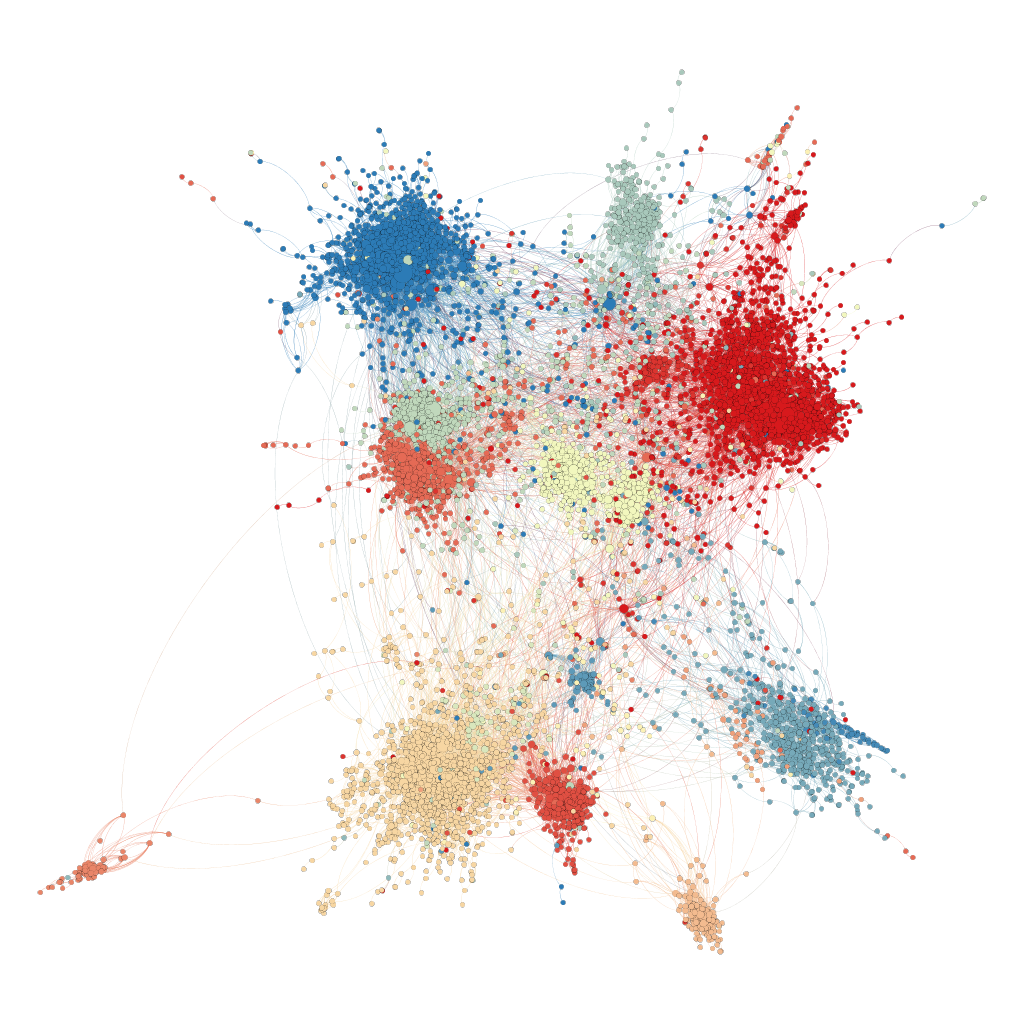
\includegraphics[width=1.097\textwidth]{img/resultados/grado-targets.png}
    \caption{Topología de la red. El color indica el país de cada usuario.}
\end{figure}

\begin{figure}[t]
    \centering
    \resizebox{0.78\columnwidth}{!}{%
    \begin{tabular}{| l | r |} 
        \hline
        \textbf{Medida} & \textbf{Valor} \\
        \Xhline{2\arrayrulewidth}
        Número de nodos \textbf{N} & 7,624 \\
        \hline
        Número de enlaces \textbf{L}	& 27,806 \\
        \hline
        Número máximo de enlaces \textbf{$L_{max}$} & 58117752 \\
        \hline
        Densidad del grafo \textbf{$L/L_{max}$} & 0.001 \\
        \Xhline{2\arrayrulewidth}
        Grado medio \textbf{<k>} & 7.294 \\
        \hline
        Diámetro \textbf{$d_{max}$} & 15 \\
        \hline
        Distancia media \textbf{d} & 5.232237269 \\
        \hline
        Coeficiente medio de clustering \textbf{<C>} & 0.285 \\
        \Xhline{2\arrayrulewidth}
        Número de componentes conexas & 1 \\
        \hline
        Número de nodos componente gigante (y \%) & 7,624 (100) \\
        \hline
        Número de aristas componente gigante (y \%) & 27,806 (100) \\
        \hline
    \end{tabular}
    }
    \caption{Medidas globales de la red.}
\end{figure} \newpage
    % \section{Análisis de Red}

% A social network of LastFM users which was collected from the public API in March 2020. Nodes are LastFM users from Asian countries and edges are mutual follower relationships between them. The vertex features are extracted based on the artists liked by the users. The task related to the graph is multinomial node classification - one has to predict the location of users. This target feature was derived from the country field for each user.

Para esta práctica se ha usado la red social \textbf{LastFMAsia}, que representa conexiones mutuas de amistad entre usuarios asiáticos de la plataforma LastFM. El dataset incluye además una variable \textit{target} que codifica el país de origen de cada uno de los usuarios, con un total de 17 opciones posibles.

LastFM es una red social centrada en el ámbito músical, donde los usuarios pueden escuchar, comentar y debatir sobre sus gustos e intereses. De forma similar a Facebook, se permiten crear comunidades y foros de debate donde compartir información.

Referencia: \url{http://snap.stanford.edu/data/feather-lastfm-social.html}

\vspace{\baselineskip}

Tenemos por tanto una red no dirigida y sin pesos, con una única componente conexa. La red se caracteriza por tener una gran dimensión pero muy baja densidad (probablemente habitual en redes de este tamaño), aunque la distancia media no es alta debido a un buen grado medio global en la red.

Apreciamos también un buen coeficiente de clustering, pero un tanto bajo para los habituales en redes sociales. Esto se puede apreciar fácilmente en la Figura 1, donde aunque la mayor parte de los nodos pertenecen a algún hub (ya sea de mayor o menor tamaño), existe un buen número de ellos que se ubican en "zonas de paso" entre países.

En la Figura 4 vemos que la tendencia a este valor un tanto bajo se ve afectada por tener un 40\% de los nodos un coeficiente muy cercano a cero.

\vspace{\baselineskip}

Sobre los grados de los nodos, contamos con una media de 7.294 y una desviación típica de 11.499. Esta media es un tanto baja en comparación con redes de amistad como Facebook, aunque en este caso al ser un red centrada en música no debería de extrañar pues es probable que los nodos no estén conectados con personas que conozcan personalmente.

En la figura ? vemos cláramente una ley de la potencia en la distribución de grados, indicándonos que tenemos una red libre de escala. Aquí se refleja mejor la alta desviación en el grado de los nodos, pues existe una buena cantidad de ellos con más de 100 enlaces.

Estos actores probablemente correspondan a creadores habituales de contenido (posts, reviews...) y sean muy influyentes en el manejo de información de la red. \newpage
    % \section{Análisis de Centralidad}

\begin{figure}[ht]
    \centerfloat
    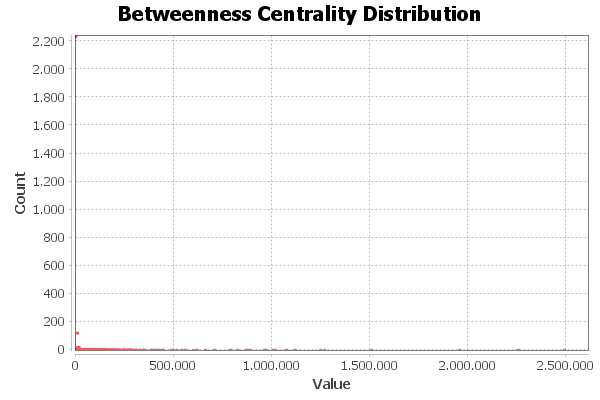
\includegraphics[width=0.9\textwidth]{img/resultados/distanciaGrafo/Betweenness Centrality Distribution.png}
    \caption{Intermediación.}
\end{figure}

\begin{figure}[ht]
    \centerfloat
    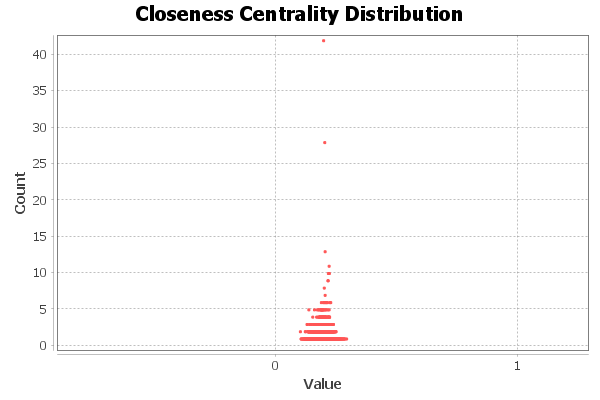
\includegraphics[width=0.9\textwidth]{img/resultados/distanciaGrafo/Closeness Centrality Distribution.png}
    \caption{Cercanía.}
\end{figure}

\begin{figure}[ht]
    \centerfloat
    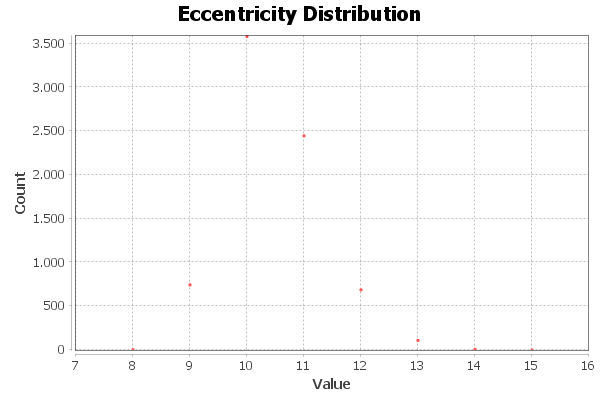
\includegraphics[width=0.9\textwidth]{img/resultados/distanciaGrafo/Eccentricity Distribution.png}
    \caption{Excentricidad.}
\end{figure}

\begin{figure}[ht]
    \centerfloat
    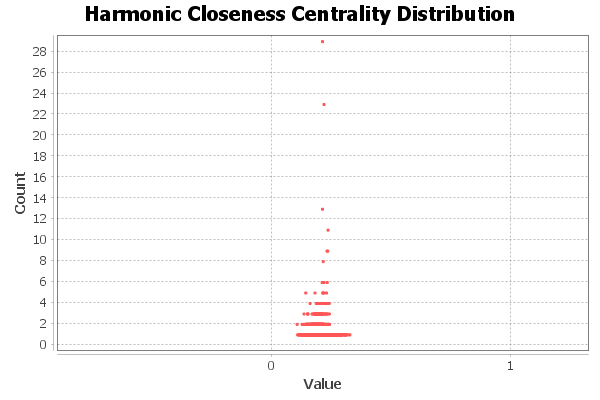
\includegraphics[width=0.9\textwidth]{img/resultados/distanciaGrafo/Harmonic Closeness Centrality Distribution.png}
    \caption{Cercanía harmónica.}
\end{figure}

\begin{figure}[t]
    \centering
    \resizebox{0.9\columnwidth}{!}{%
    \begin{tabular}{| l | l | l | l |} 
        \hline
        \textbf{Centralidad de Grado} & \textbf{Intermediación} & \textbf{Cercanía} & \textbf{Vector propio} \\
        \Xhline{2\arrayrulewidth}
        \textbf{7237} - 216 & 	\textbf{7199} - 2,612,617 & \textbf{7199} - 0.2907 & 	\textbf{7237} - 1.0000  \\
        \hline
        \textbf{3530} - 175 & 	\textbf{7237} - 2,486,453 & 	\textbf{7237} - 0.2856 & \textbf{3240} - 0.7149  \\
        \hline
        \textbf{4785} - 174 & 	\textbf{2854} - 2,253,302 & 	\textbf{4356} - 0.2816 & 	\textbf{3597} - 0.7052  \\
        \hline
        \textbf{524}   - 172 & 	\textbf{4356} - 1,953,690 & 	\textbf{2854} - 0.2803 & 	\textbf{763}   - 0.6555  \\
        \hline
        \textbf{3450} - 159 & \textbf{6101} - 1,504,994 & 	\textbf{5454} - 0.2798 & 	\textbf{2083} - 0.5940  \\
        \hline
    \end{tabular}
    }
    \caption{Tabla de actores más relevantes.}
\end{figure}

\begin{figure}[ht]
    \centerfloat
    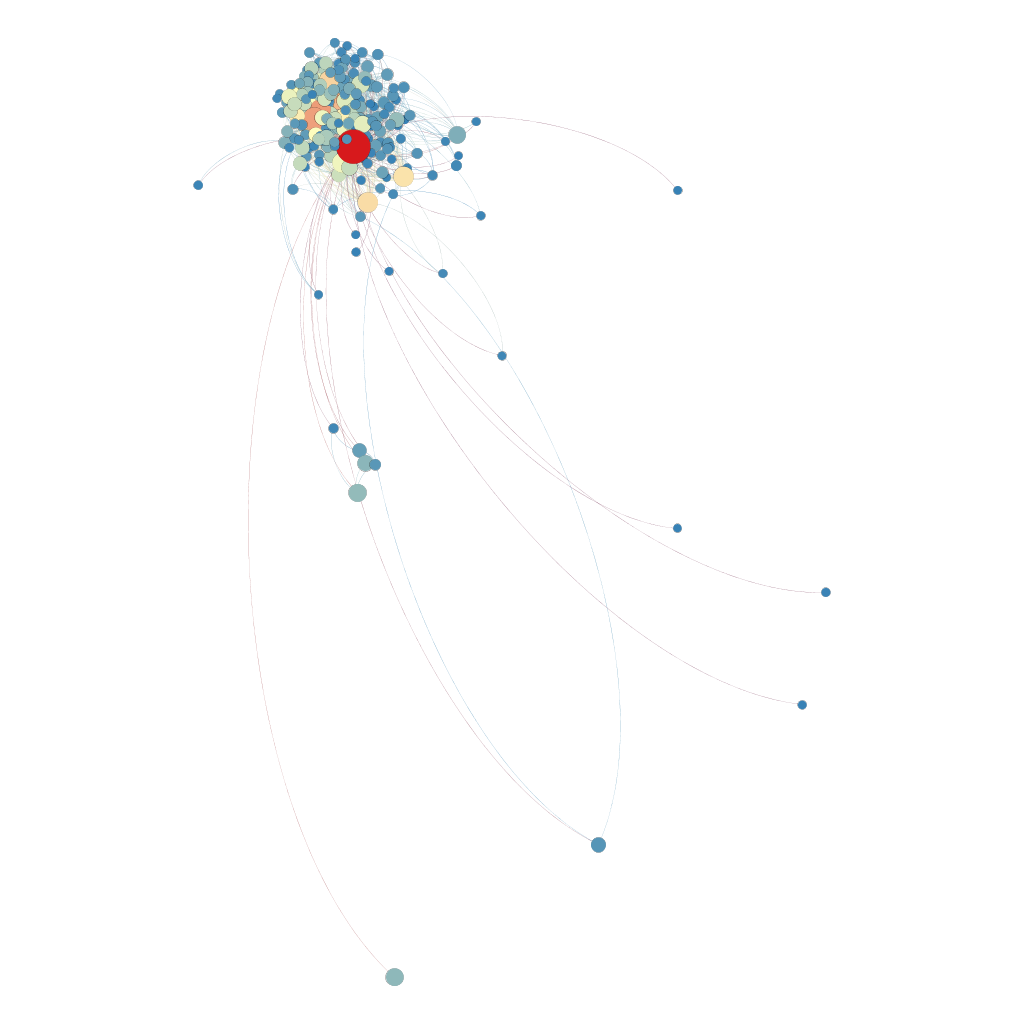
\includegraphics[width=0.9\textwidth]{img/resultados/grado-vector7237.png}
    \caption{Vecinos del nodo 7237. A mayor grado mayor tamaño, más rojo mayor valor de vector propio.}
\end{figure}

\begin{figure}[ht]
    \centerfloat
    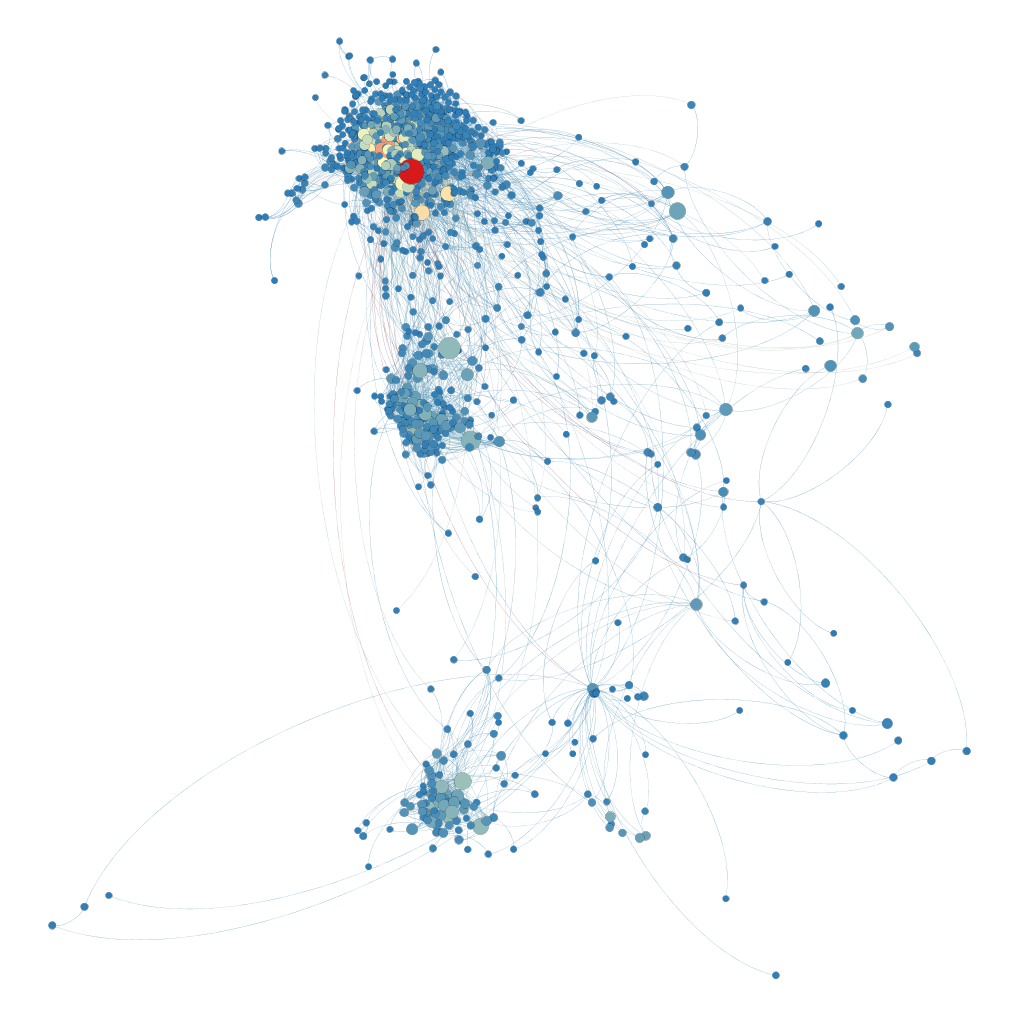
\includegraphics[width=0.9\textwidth]{img/resultados/grado-vector7237-prof2.png}
    \caption{Vecinos del nodo 7237 a profundidad 2.}
\end{figure}

\begin{figure}[ht]
    \centerfloat
    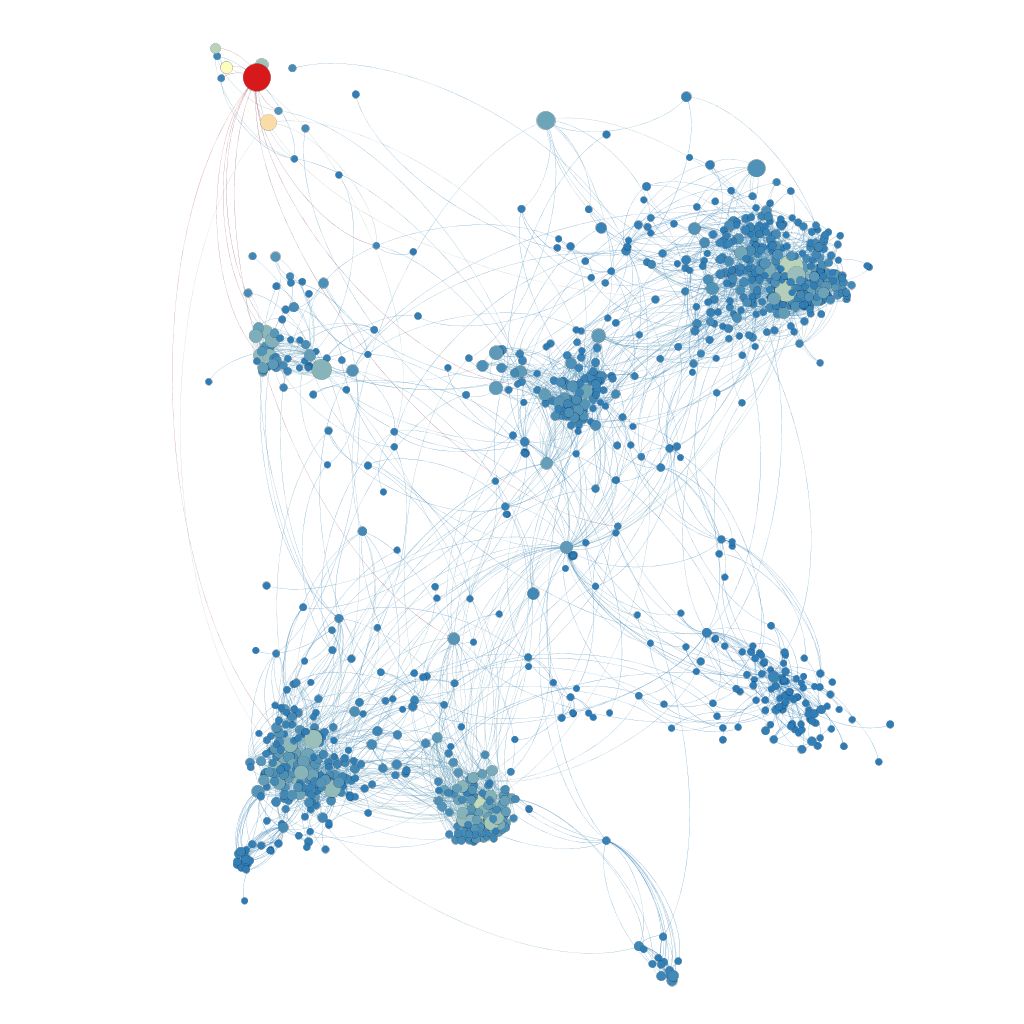
\includegraphics[width=0.9\textwidth]{img/resultados/grado-vector7199-prof2.png}
    \caption{Vecinos del nodo 7199 a profundidad 2.}
\end{figure}

\begin{figure}[ht]
    \centerfloat
    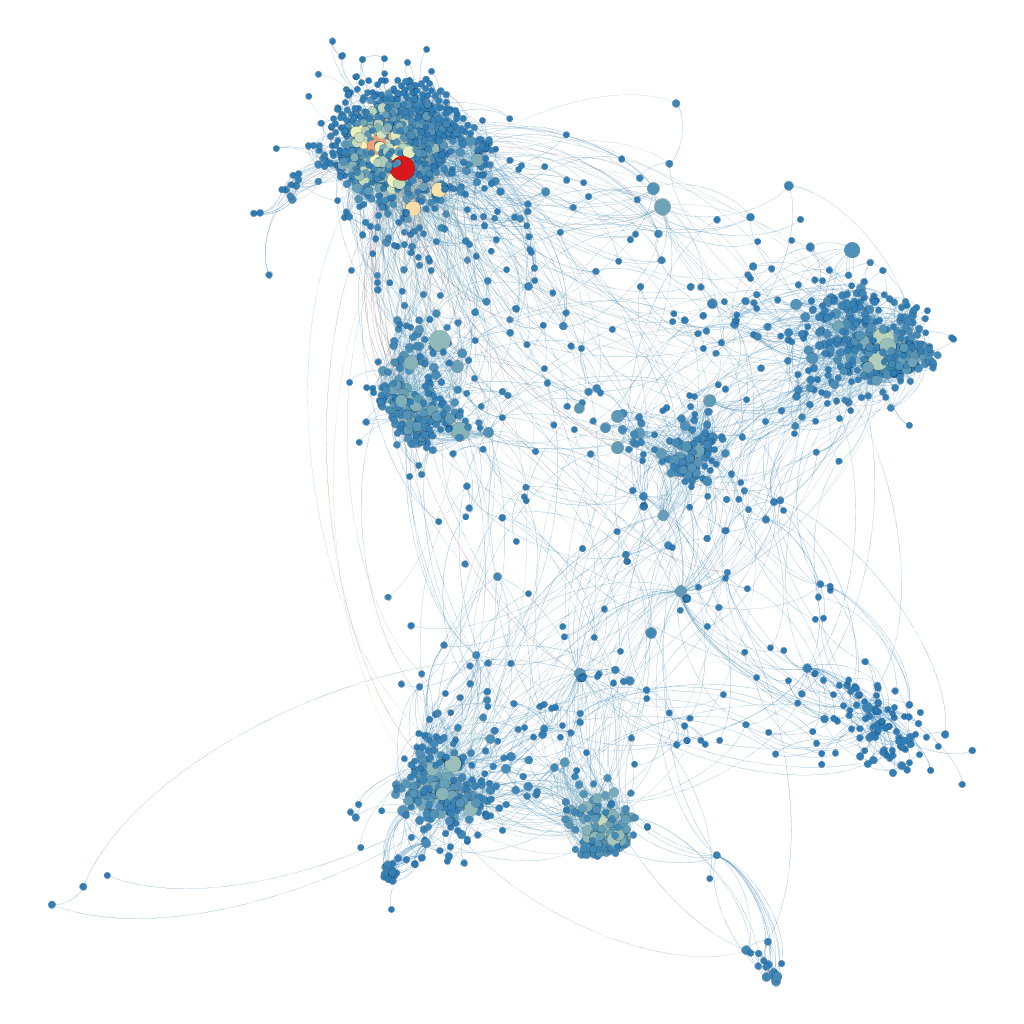
\includegraphics[width=0.9\textwidth]{img/resultados/grado-vector7199y7237.png}
    \caption{Unión de los vecinos del nodo 7237 y del 7199 a profundidad 2.}
\end{figure}

Los valores de la Figura 10 carecen de significado si no nos fijamos en sus gráficas de distribución.

Respecto a la centralidad, como se comentó anteriormente estos outliers es muy probable que correspondan a creadores de contenido, ya que sus valores se encuentran extremadamente separados de la media en la red.

Acerca de la intermediación, vemos en la Figura 6 que la variación en la distribución es enorme, donde la mayoría de nodos se ubica por debajo de los 250,000. Este resultado no es extraño, el grado medio es relativamente bajo en esta red de amistad, por lo que solo un porcentaje pequeño de los nodos hacen de conexiones entre las diferentes comunidades.

\vspace{\baselineskip}

Hacemos notar que los nodos con buena alta intermediación tienen también los valores más altos de cercanía. No nos queda del todo claro cuál puede ser el motivo tras ello, pero es probable que estos nodos estén áltamente conectados con dos o más hubs en la red, tal y como muestra la  Figura ?? % (13, vecinos de 7199)

\vspace{\baselineskip}

Por último, nos fijamos en los valores de vector propio tras 100 iteraciones. Es de destacar una alta diferencia entre el primer actor (7237) respecto del resto, además contando con un valor de 1. Esto nos indica que la ubicación en la que se ubica en la red es muy buena, y no resulta extraño encontrarnos enlaces con 3240, 3597 y 2083, también tres de los actores con mayor valor de vector propio.

En la Figura ? se muestran los vecinos a profundidad uno y dos del nodo 7237. Vemos que ya de por sí las conexiones del actor son buenas pero además a partir de sus enlaces es capaz de extenderse a la zona más remota de la red (la inferior izquierda en la Figura 1).

\vspace{\baselineskip}

En la Figura ? vemos la unión de los vecinos a profundidad dos del par de nodos 7237-7199. Destacamos dos cosas de esta figura: por un lado, la gran importancia de estos actores puesto que con un máximo de dos enlaces alcanzamos un 26.3\% de la red (2043 nodos), y por otra parte la influencia en el flujo de información ya que sabemos que \textbf{en media} añadiéndole solo cuatro enlaces más (para un total de seis) podemos transmitir a toda la red.

Estos hechos se hacen notar respectivamente en los altos valores de cercanía (una buena parte de los nodos se conectan a estos dos en pocos saltos) e intermediación (hacen de enlace entre varias comunidades).  \newpage
    % \section{Estudio de las Comunidades}

\begin{figure}
  \centering  
  \begin{subfigure}[t]{0.48\textwidth}
    \centering
    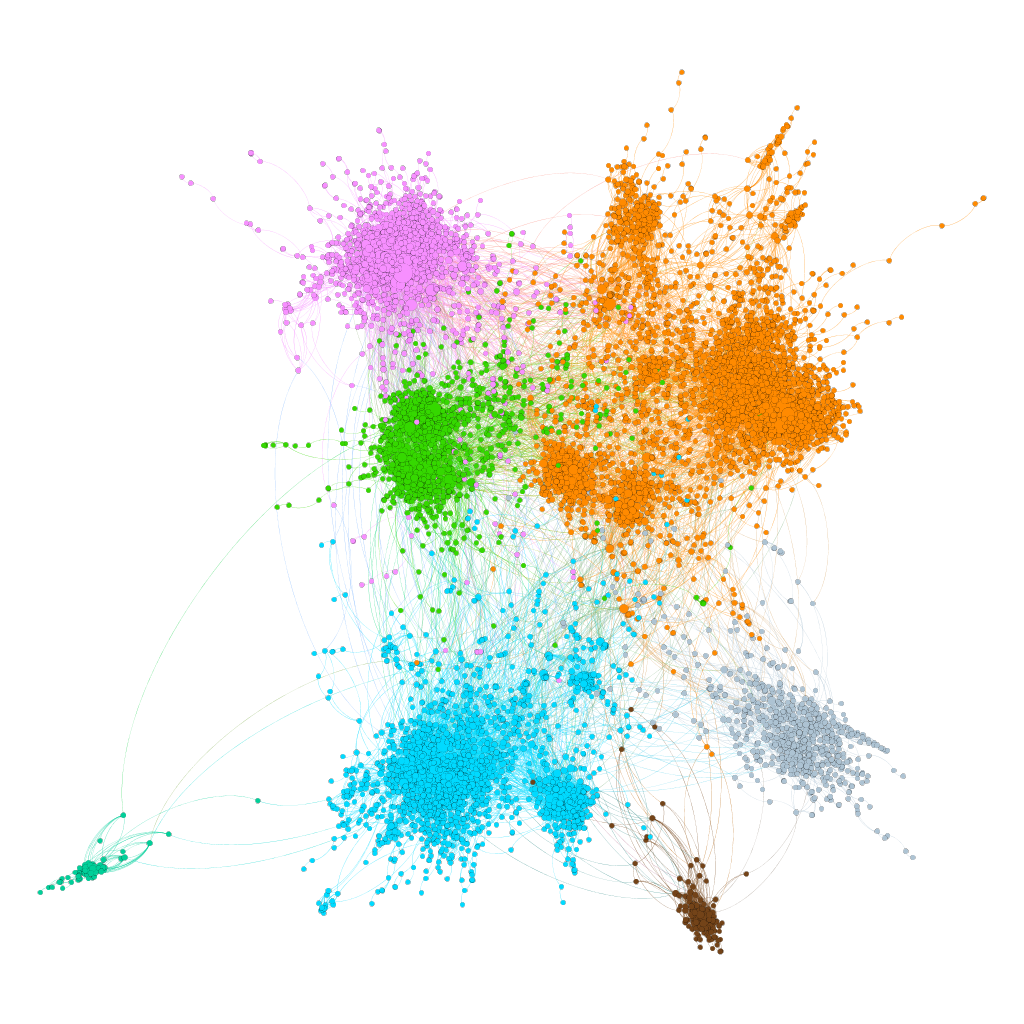
\includegraphics[width=\textwidth]{img/resultados/grado-leinen0.1.png}
    \caption{Coeficiente 0.1.}
  \end{subfigure}
  \vspace{7mm}
  \hfill
  \begin{subfigure}[t]{0.48\textwidth}
    \centering
    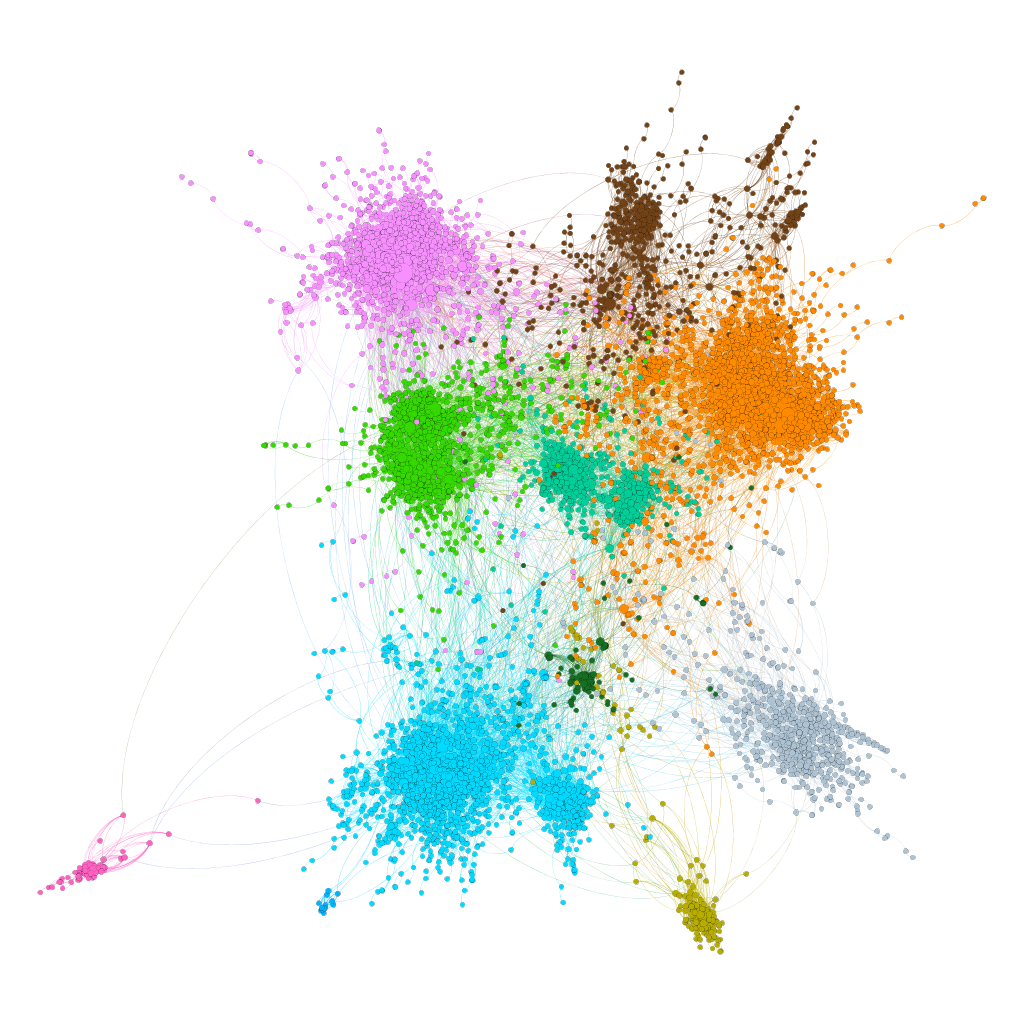
\includegraphics[width=\textwidth]{img/resultados/grado-leinen0.25.png}
    \caption{Coeficiente 0.25.}
  \end{subfigure}
  \hfill
  \begin{subfigure}[t]{0.48\textwidth}
    \centering
    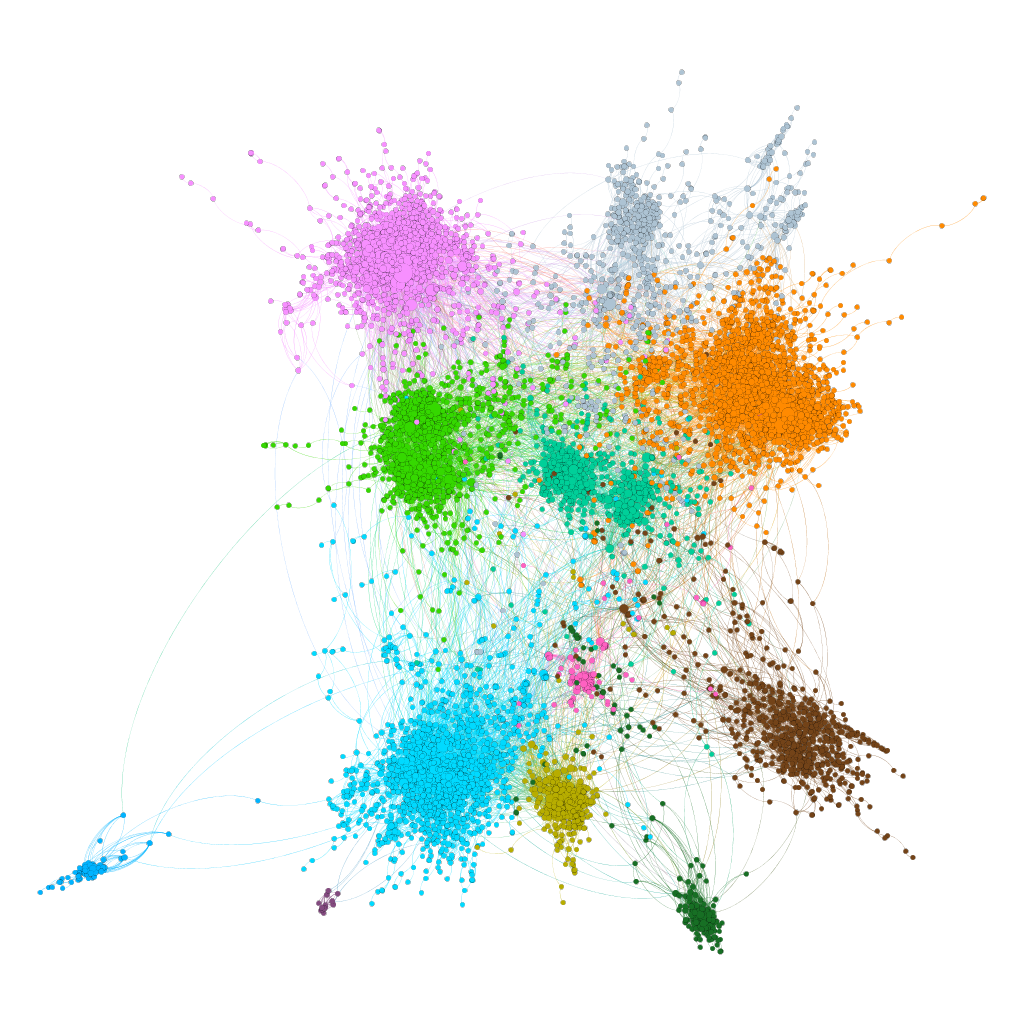
\includegraphics[width=\textwidth]{img/resultados/grado-leinen0.33.png}
    \caption{Coeficiente 0.33.}
  \end{subfigure}
  \hfill
  \begin{subfigure}[t]{0.48\textwidth}
    \centering
    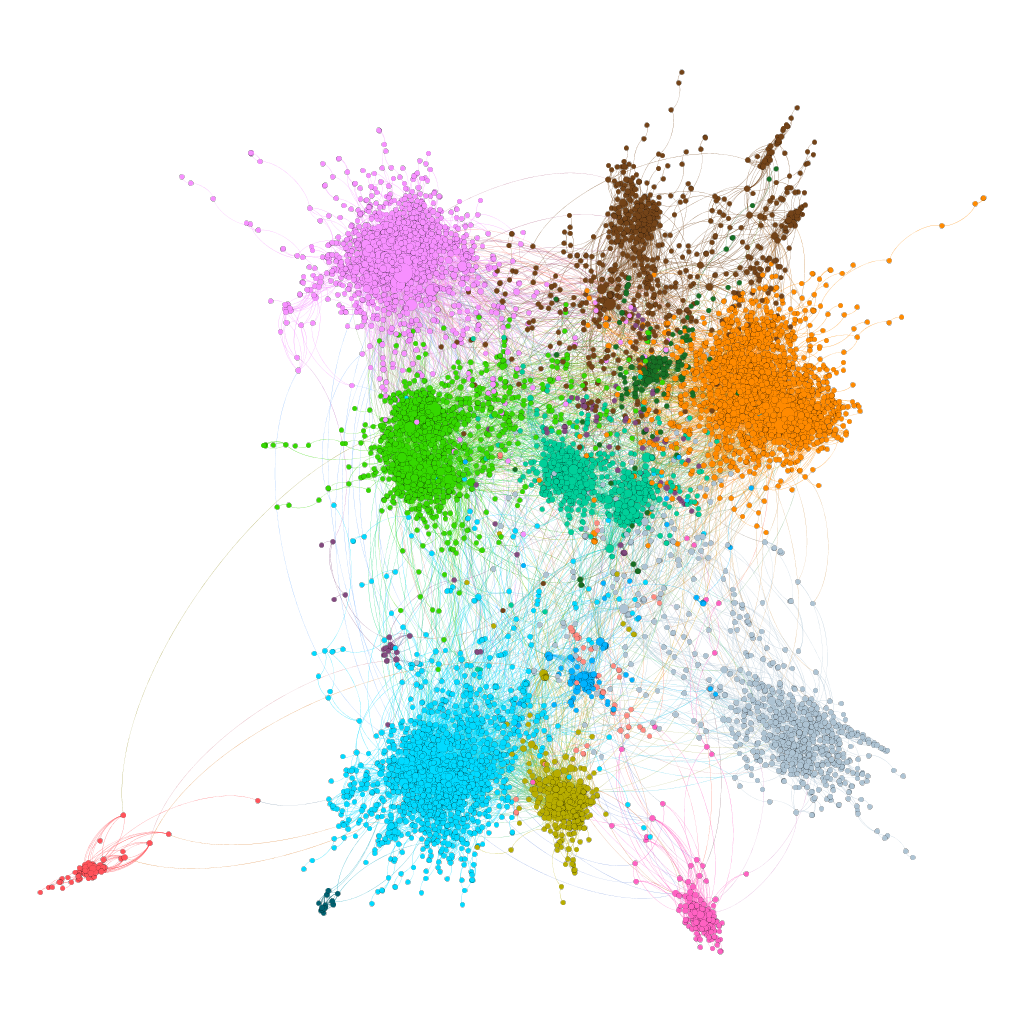
\includegraphics[width=\textwidth]{img/resultados/grado-leinen0.5.png}
    \caption{Coeficiente 0.5.}
  \end{subfigure}

  \caption{Comunidades detectadas por el algoritmo Leinen para diferentes coeficientes.}
\end{figure}

\begin{figure}
    \centering  
    \begin{subfigure}[t]{0.48\textwidth}
      \centering
      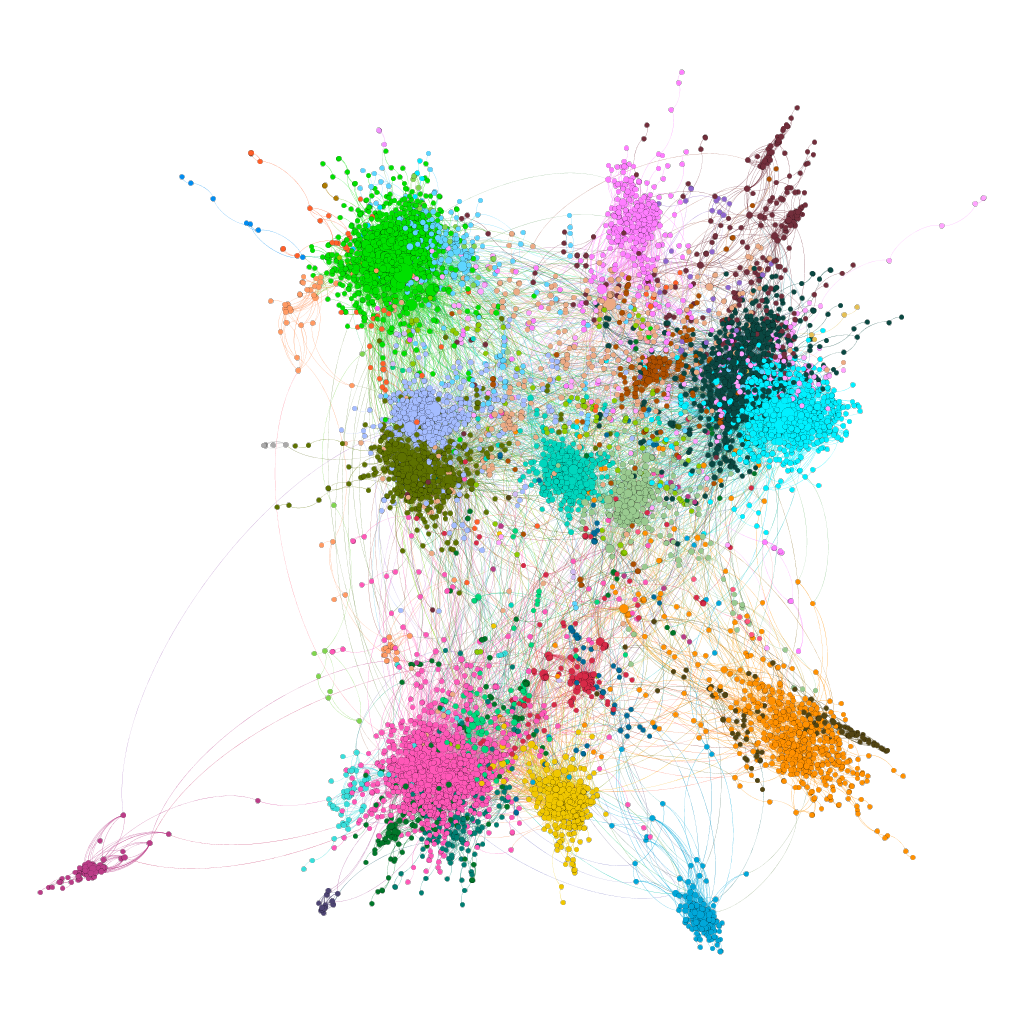
\includegraphics[width=\textwidth]{img/resultados/grado-lovaina0.5.png}
      \caption{Coeficiente 0.5.}
    \end{subfigure}
    \vspace{7mm}
    \hfill
    \begin{subfigure}[t]{0.48\textwidth}
      \centering
      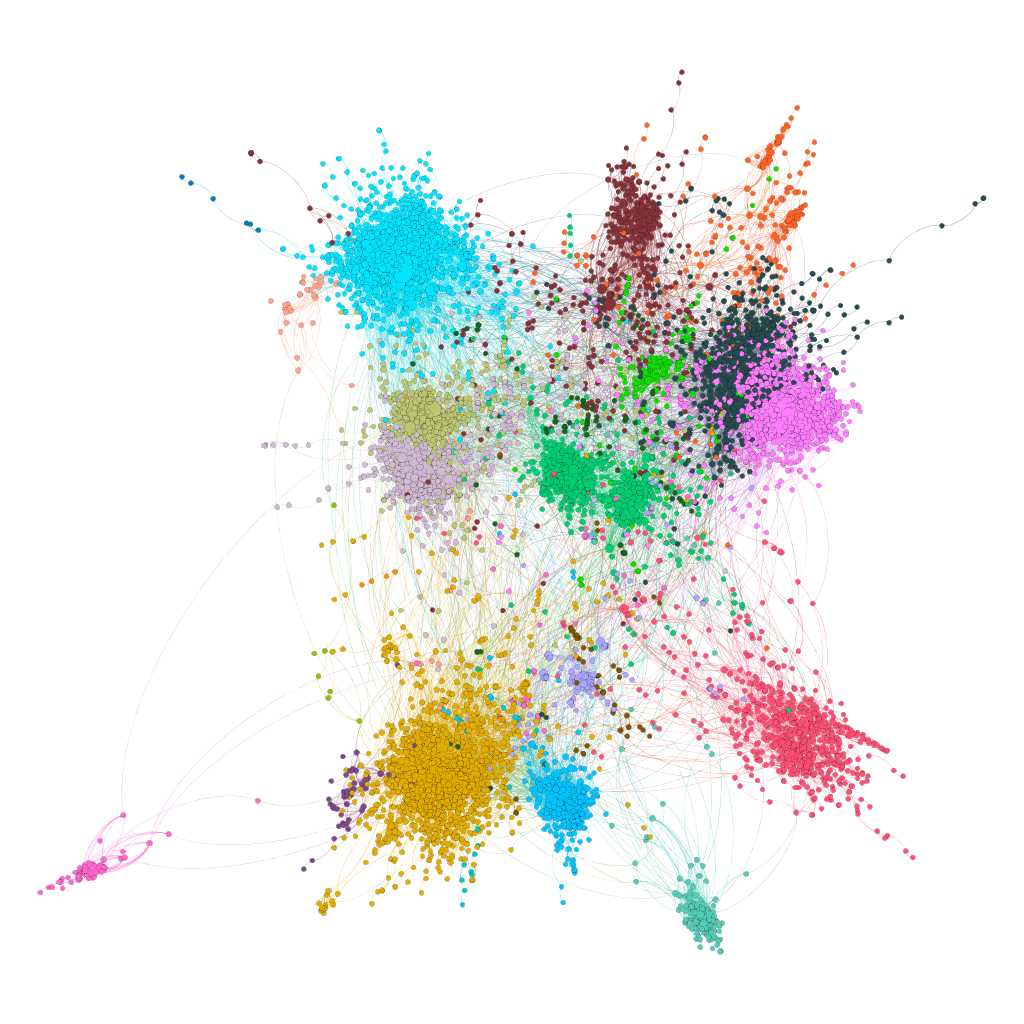
\includegraphics[width=\textwidth]{img/resultados/grado-lovaina1.png}
      \caption{Coeficiente 1.}
    \end{subfigure}
    \hfill
    \begin{subfigure}[t]{0.48\textwidth}
      \centering
      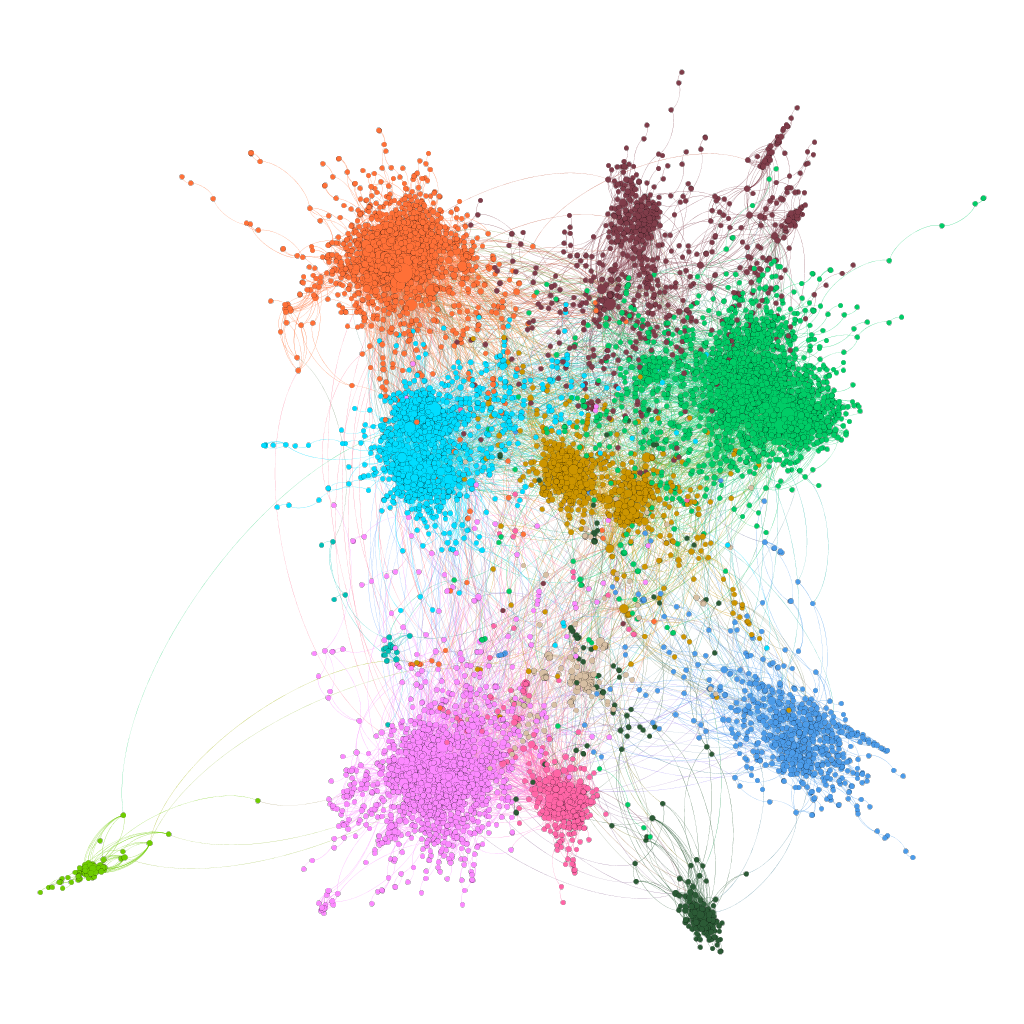
\includegraphics[width=\textwidth]{img/resultados/grado-lovaina2.png}
      \caption{Coeficiente 2.}
    \end{subfigure}
    \hfill
    \begin{subfigure}[t]{0.48\textwidth}
      \centering
      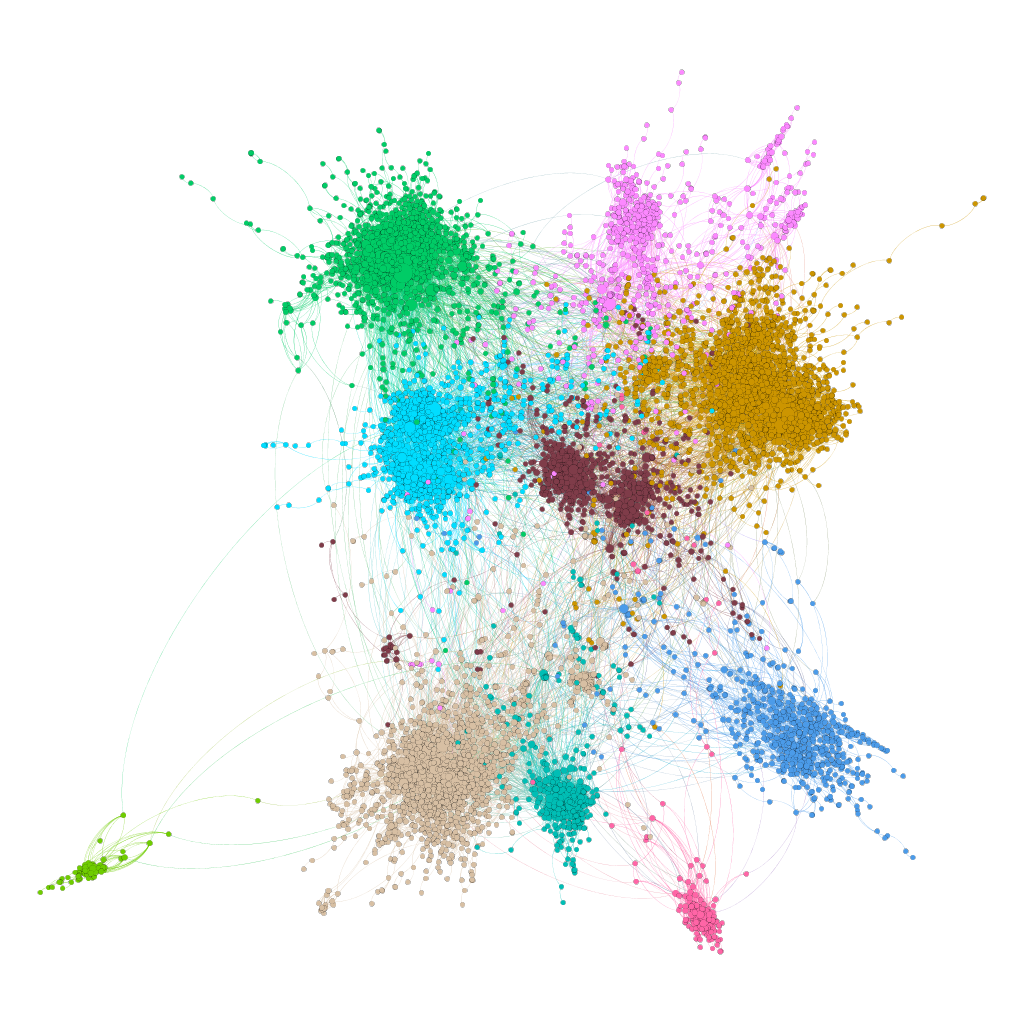
\includegraphics[width=\textwidth]{img/resultados/grado-lovaina3.png}
      \caption{Coeficiente 3.}
    \end{subfigure}
  
    \caption{Comunidades detectadas por el algoritmo Lovaina para diferentes coeficientes.}
\end{figure}

\begin{figure}
  \centering  
  \begin{subfigure}[t]{0.48\textwidth}
    \centering
    \includegraphics[width=\textwidth]{img/resultados/lovaina0.5/communities-size-distribution.png}
    \caption{Coeficiente 0.5.}
  \end{subfigure}
  \vspace{7mm}
  \hfill
  \begin{subfigure}[t]{0.48\textwidth}
    \centering
    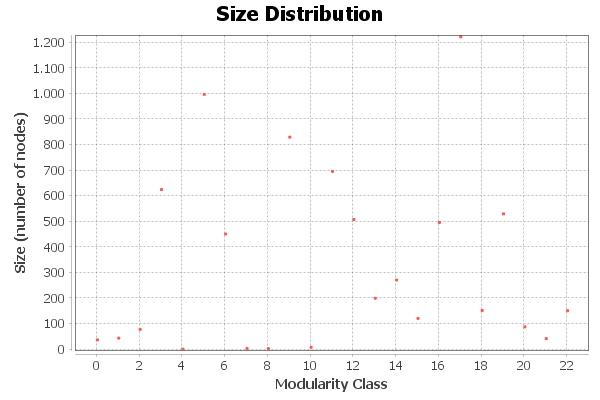
\includegraphics[width=\textwidth]{img/resultados/lovaina1/communities-size-distribution.png}
    \caption{Coeficiente 1.}
  \end{subfigure}
  \hfill
  \begin{subfigure}[t]{0.48\textwidth}
    \centering
    \includegraphics[width=\textwidth]{img/resultados/lovaina2/communities-size-distribution.png}
    \caption{Coeficiente 2.}
  \end{subfigure}
  \hfill
  \begin{subfigure}[t]{0.48\textwidth}
    \centering
    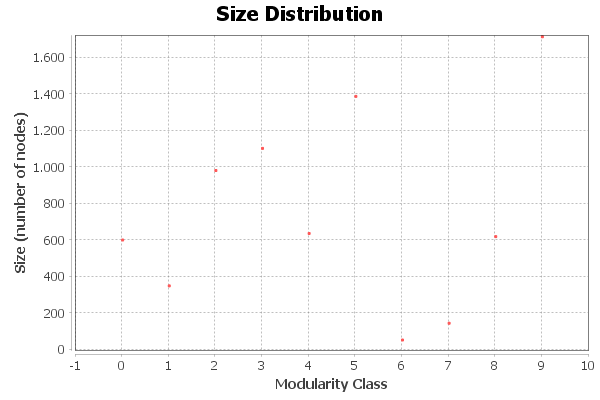
\includegraphics[width=\textwidth]{img/resultados/lovaina3/communities-size-distribution.png}
    \caption{Coeficiente 3.}
  \end{subfigure}

  \caption{Gráfico de distribuciones para el algoritmo Lovaina en diferentes coeficientes.}
\end{figure}

\vspace{2\baselineskip}

\begin{figure}[H]
  \centering
  \resizebox{0.75\columnwidth}{!}{%
  \begin{tabular}{| l | c || c | c |} 
      \hline
      \textbf{Algoritmo} & \textbf{Coeficiente} & \textbf{Modularidad} & \textbf{Clústers}  \\
      \Xhline{2\arrayrulewidth}
      \multirow{4}{*}{Leinen} 
        & 0.1 & 0.941 & 7 \\ \cline{2-4}
        & 0.25 & 0.913 & 11 \\ \cline{2-4}
        & 0.33 & 0.901 & 11 \\ \cline{2-4}
        & 0.5 & 0.878 & 15 \\ \cline{2-4}
      \hline
      \multirow{4}{*}{Lovaina} 
        & 0.5 & 0.800 & 42 \\ \cline{2-4}
        & 1 & 0.813 & 23 \\ \cline{2-4}
        & 2 & 0.806 & 12 \\ \cline{2-4}
        & 3 & 0.803 & 10 \\ \cline{2-4}
      \hline
  \end{tabular}
  }
  \caption{Modularidad y número de clústers obtenido por cada algoritmo.}
\end{figure}

\newpage

La referencia sobre los países puede ser un buen comienzo de partida para la búsqueda de buenas comunidades, pero es importante no dejarse engañar por esto pues existen hubs de diferentes regiones altamente conectados entre sí. Además, algunas de las fronteras entre los hubs de los países son difusas y existen zonas de baja conectividad fuertemente entremezcladas.

El objetivo de la búsqueda de comunidades es después de todo encontrar grupos de usuarios con intereses comunes que nos permitan simplificar el manejo de la red y la transmisión de información. La ubicación regional probablemente sea relevante en la semántica de nuestra red pero no debe ser el factor decisivo para una selección correcta de comunidades.

\vspace{\baselineskip}

A partir de la estructura de la red vemos que la zona central y superior del grafo no muestra una estructura modular clara. Por el contrario, la zona inferior muestra más claramente una partición en un mínimo de cuatro o cinco comunidades, y esto es detectado perfectamente por el método Leinen independientemente del coeficiente, pero no tanto por Lovaina, donde es necesario empujar el coeficiente hacia arriba para separar mejor estos hubs.

\vspace{\baselineskip}

En cuanto a los efectos en la modularidad y el número de clústers que muestra la Figura 18, nos fijamos en que la calidad de las particiones con Lovaina no varía de manera substancial, aunque sí lo hace el número de clústers que forma.

\vspace{\baselineskip}

Sobre las comunidades en sí, visualmente concluímos que un número de diez parece adecuado para esta red, tal y como se consigue en la Figura 16.d. De esta forma contaríamos con cinco clústers bien diferenciados en la parte inferior conectándose a un núcleo central a su vez dividido en cuatro. Este núcleo contaría con la mayoría de nodos de la red fuertemente interconectados entre sí. Por último, nos quedaría un hub denso en la parte superior izquierda con muchas conexiones al núcleo grande.

\vspace{\baselineskip}

En referencia al significado semántico de estas comunidades, es de esperar que los usuarios se agrupen por estilos y géneros de música favoritos donde los intercambios de información vayan sobre esos temas. 

Con una partición en diez podríamos suponer que en el núcleo central predominan los géneros de moda en la cultura asiática actual (la red se construyó en 2020), como es el K-Pop, el J-Pop y el C-Pop, y que en las comunidades inferiores predominan estilos relacionados con estos géneros pero de ámbito menos popular, como el rock, el rap o el pop anglosajón.

Por último, tendríamos un hub interesante en la esquina inferior izquierda, conectándose al resto de la red por muy pocos nodos. Este hub nos podría dar información sobre los géneros menos relevantes en la comunidad, como podría ser el metal, el jazz, o la electrónica. \newpage
    % \section{Anexos}

\begin{figure}[ht]
    \centering
    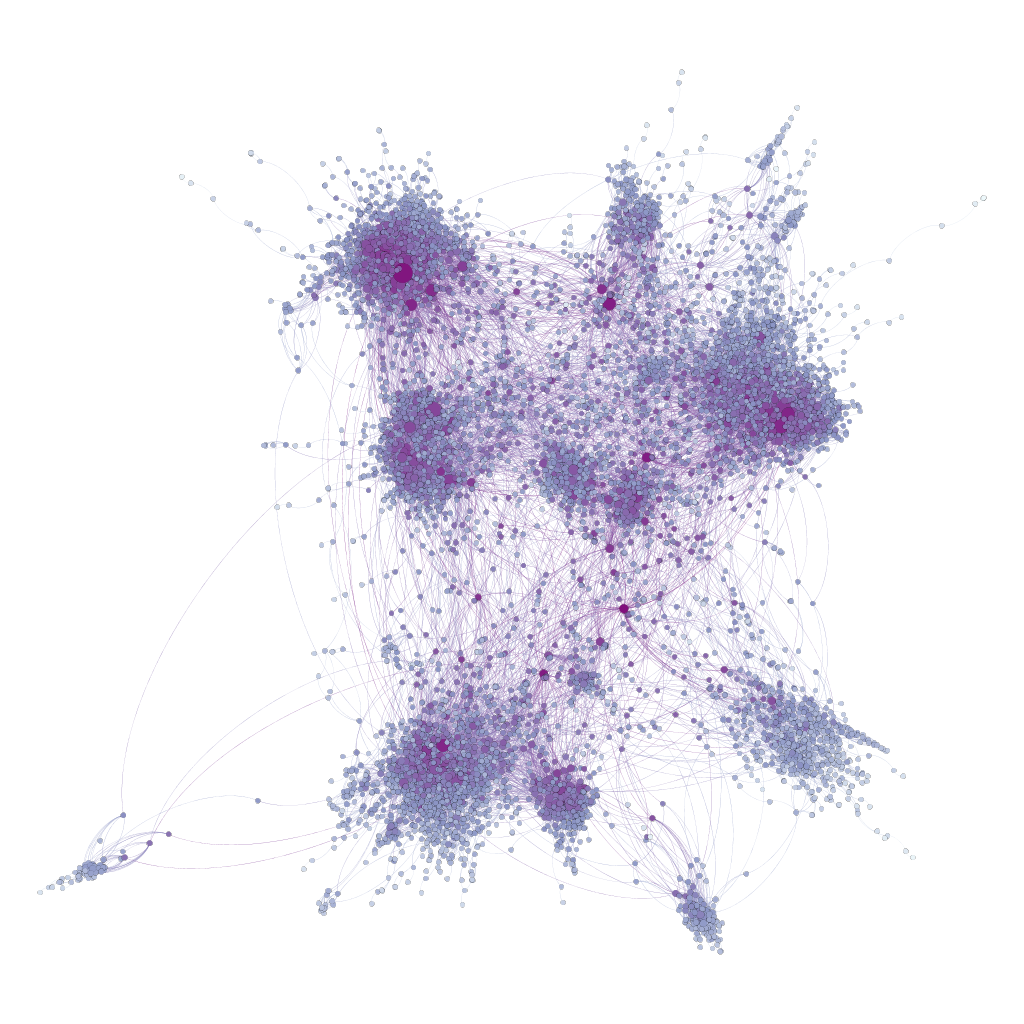
\includegraphics[width=1\textwidth,angle=90]{img/resultados/grado-cercania.png}
    \caption{A mayor tamaño de nodo mayor grado. Mayor intensidad de violeta implica mayor cercanía.}
\end{figure}

\begin{figure}[ht]
    \centering
    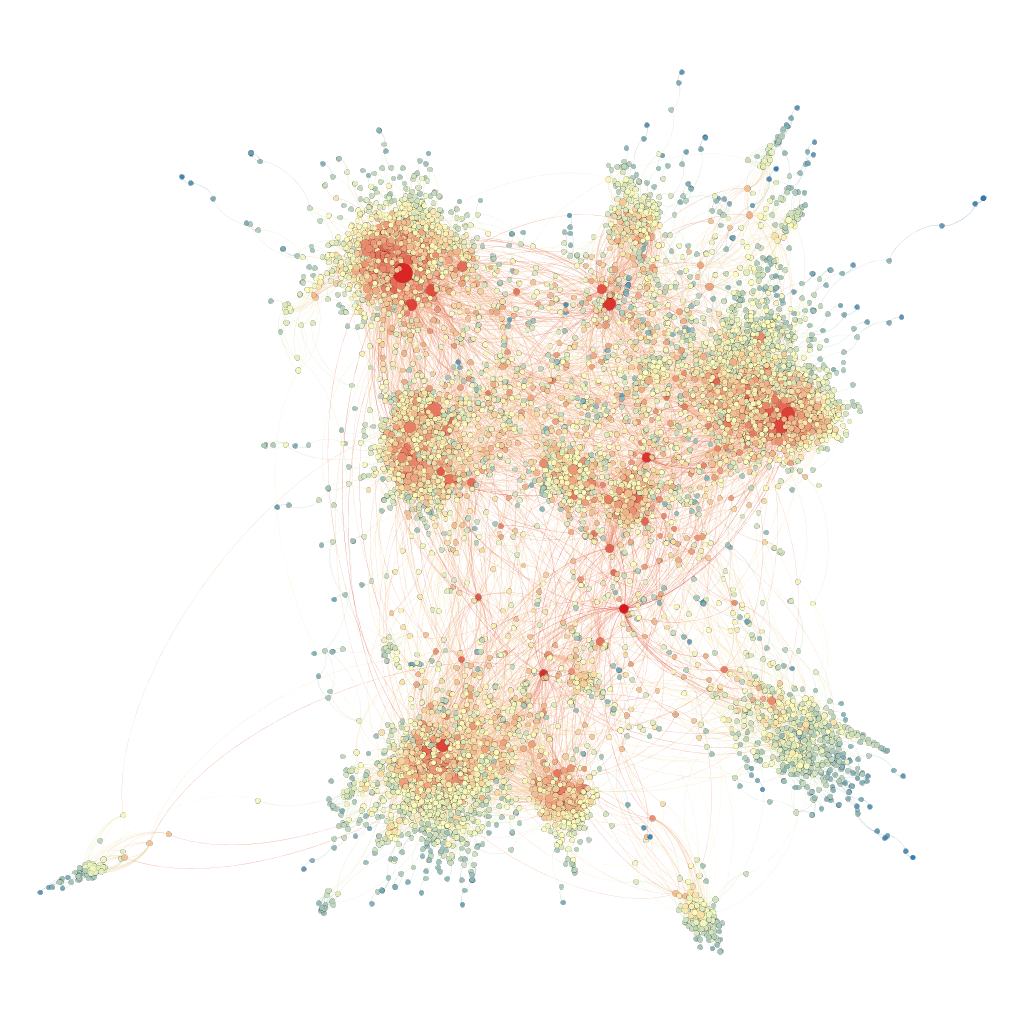
\includegraphics[width=1\textwidth,angle=90]{img/resultados/grado-cercania2.png}
    \caption{A mayor tamaño de nodo mayor grado. Azul implica menor cercanía, rojo más.}
\end{figure}

\begin{figure}[ht]
    \centering
    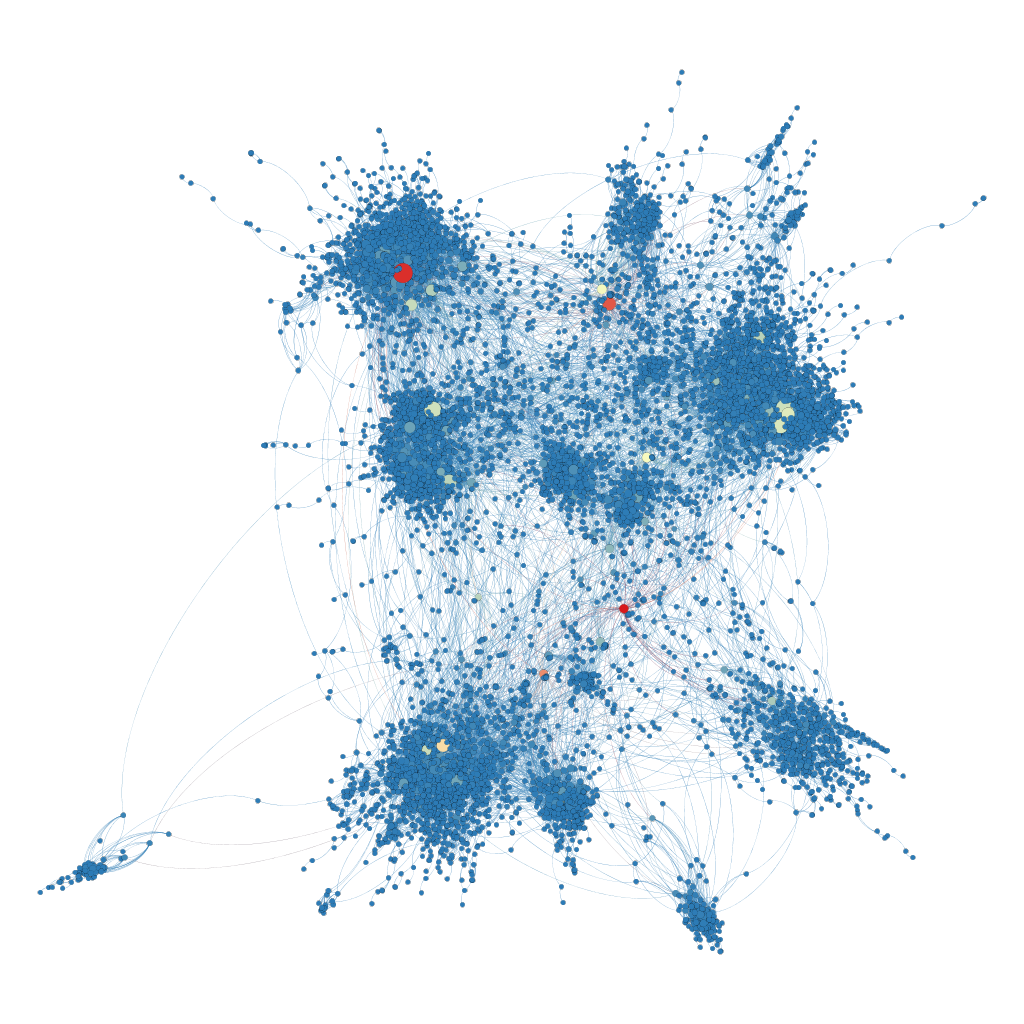
\includegraphics[width=1\textwidth,angle=90]{img/resultados/grado-intermediacion.png}
    \caption{A mayor tamaño de nodo mayor grado. Azul implica menor intermediación, rojo más.}
\end{figure}

\begin{figure}[ht]
    \centering
    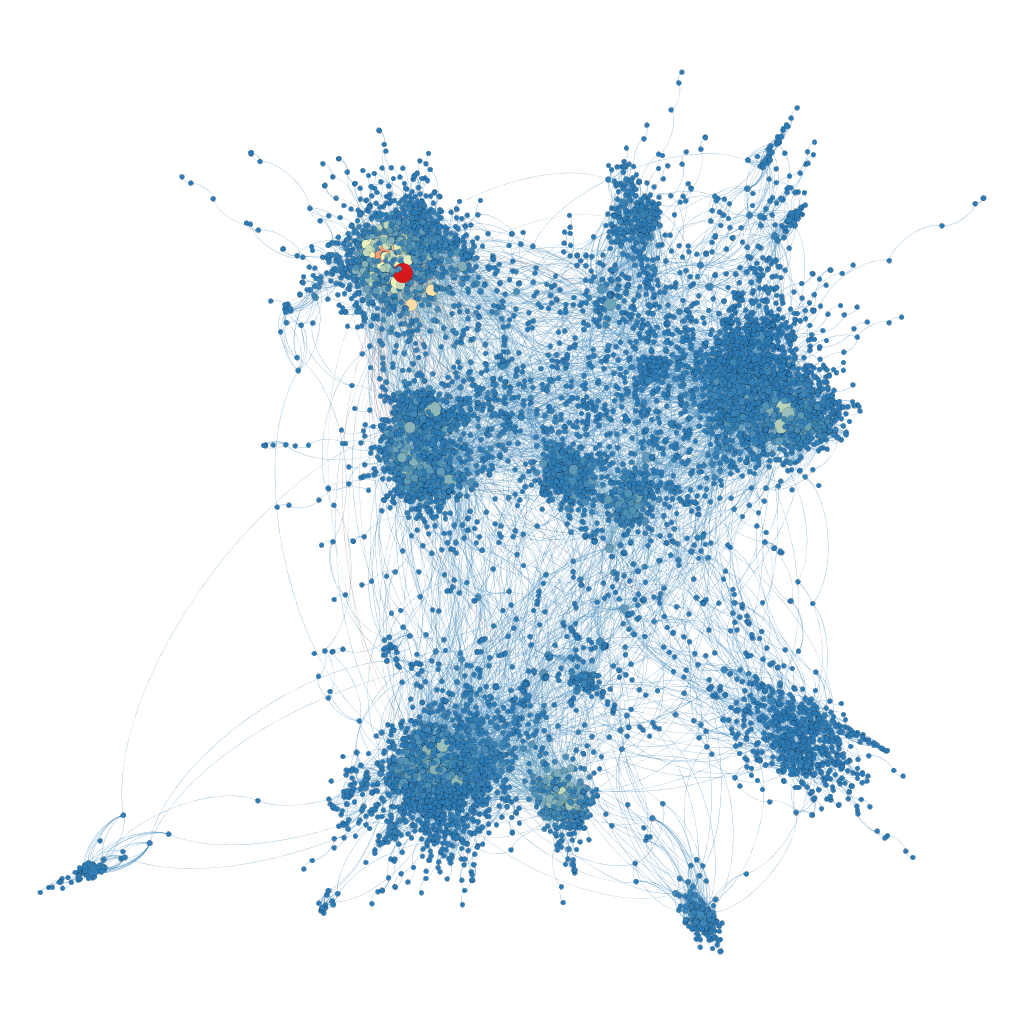
\includegraphics[width=1\textwidth,angle=90]{img/resultados/grado-vectorPropio.png}
    \caption{A mayor tamaño de nodo mayor grado. Azul implica menor vector propio, rojo más.}
\end{figure}

\begin{figure}[ht]
    \centering
    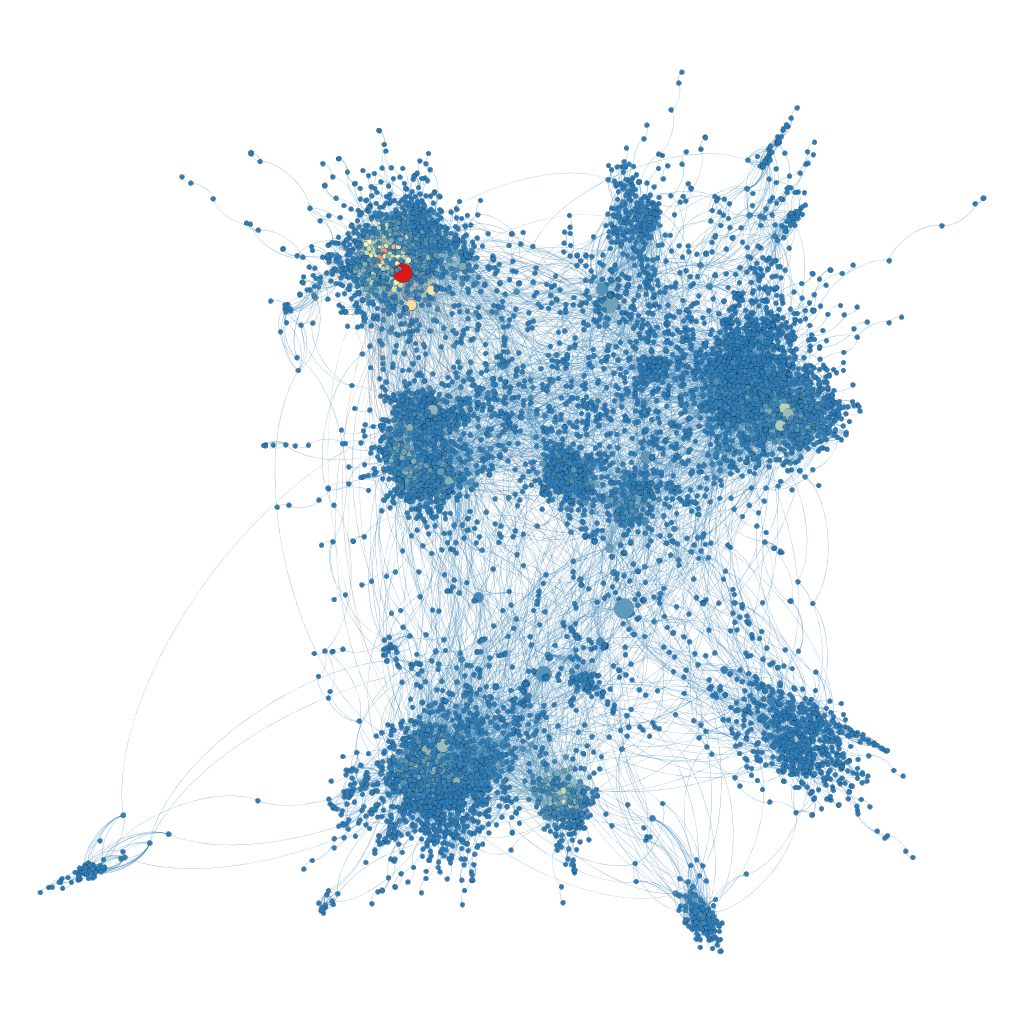
\includegraphics[width=1\textwidth,angle=90]{img/resultados/intermediacion-vectorPropio.png}
    \caption{A mayor tamaño de nodo mayor intermediación. Azul implica menor vector propio, rojo más.}
\end{figure} \newpage

    % ==============================================================================

    \setlength{\parskip}{1em}
    \newpage
    % \nocite{*}
    % \bibliography{bibliografia}
	% \bibliographystyle{plain}
\end{document}

% ==============================================================================
% ==============================================================================